\documentclass{article}
\usepackage[margin=1in]{geometry}
\usepackage{tikz}
\usetikzlibrary{shapes.geometric, arrows, positioning}
%For tikz node diagram setup
\tikzset{trapezium stretches=true}
\tikzstyle{source} = [rectangle, rounded corners, minimum width= 2cm, minimum height = 1cm, text = white, text centered, fill = black!60]
\tikzstyle{input} = [trapezium, trapezium left angle=50, trapezium right angle = 130, minimum width = 1.5cm, minimum height=1cm, text centered, text=white, fill=green!60!black]
\tikzstyle{routing} = [diamond, minimum width=2cm, minimum height=1cm, aspect = 2, text width = 2cm, text centered, text=white,fill = blue!70!black]
\tikzstyle{processor} = [rectangle, minimum width = 2cm, minimum height = 1cm, text width = 3cm, text = white, fill = purple!55!blue!40!black]
\tikzstyle{cable} = [thick, ->, >=latex]
\tikzstyle{usb} = [thick, <->, >=latex]

\renewcommand{\familydefault}{\sfdefault} %sans font for computer screens

\begin{document}
\centering
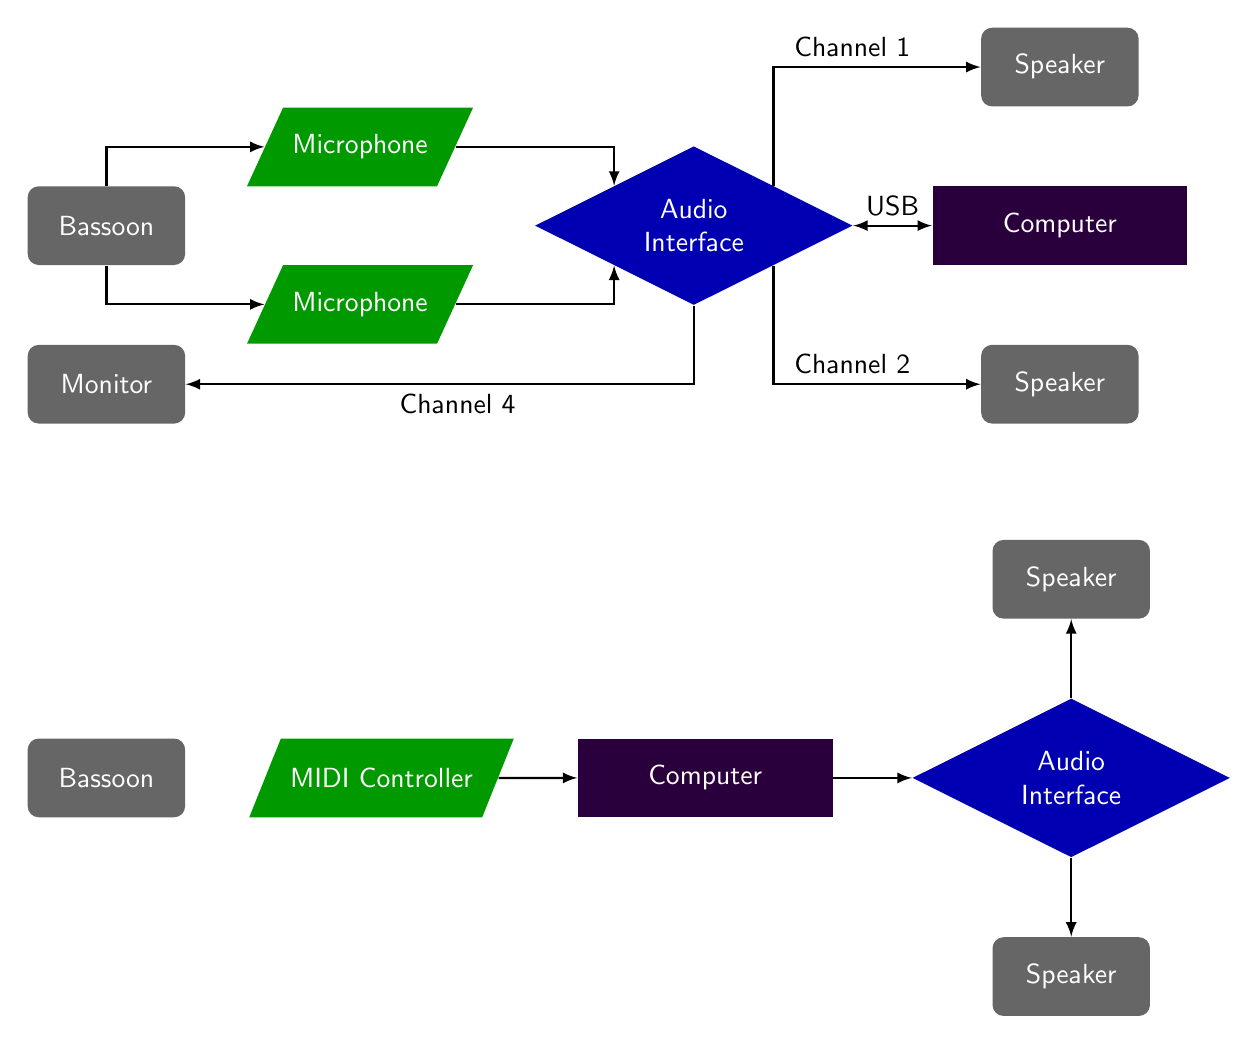
\begin{tikzpicture}[align=center,node distance = 1cm]
  \node (bsn) [source] {Bassoon};
  \node (mic1) [input, right= of bsn, yshift = 1cm] {Microphone};
  \node (mic2) [input, right= of bsn, yshift = -1cm] {Microphone};
  \draw [cable] (bsn) |- (mic1);
  \draw [cable] (bsn) |- (mic2);
  \node (interface) [routing, right = of mic1, yshift = -1cm] {Audio Interface};
  \draw [cable] (mic1) -| (interface.north west);
  \draw [cable] (mic2) -| (interface.south west);
  \node (computer) [processor, text width = 3cm, right = of interface] {Computer};
  \draw [usb] (interface) -- node[anchor = south] {USB} (computer);
  \node (speaker1) [source, above = of computer] {Speaker};
  \node (speaker2) [source, below = of computer] {Speaker};
  \draw [cable] (interface.north east) |- node[anchor=south, xshift=1cm]{Channel 1}(speaker1);
  \draw [cable] (interface.south east) |- node[anchor=south, xshift=1cm]{Channel 2}(speaker2);
  \node (monitor) [source, below = of bsn] {Monitor};
  \draw [cable] (interface.south) |- node[anchor=north, xshift=-3cm]{Channel 4}(monitor);
  %Setup 2
  \node (bsn2) [source, below= of bsn, yshift = -5cm] {Bassoon};
  \node (midi) [input, right= of bsn2] {MIDI Controller};
  \node (computer2) [processor, text width = 3cm, right= of midi] {Computer};
  \draw [cable] (midi) -- (computer2);
  \node (interface2) [routing, right = of computer2]{Audio Interface};
  \draw [cable] (computer2) -- (interface2);
  \node (speaker3) [source, above = of interface2] {Speaker};
  \node (speaker4) [source, below = of interface2] {Speaker};
  \draw [cable] (interface2.north) -- (speaker3);
  \draw [cable] (interface2.south) -- (speaker4);
\end{tikzpicture}

\end{document}